\item \textbf{{[}ALVL/9597/2015/P1/Q3{]} }

When buying software. the purchaser is issued with a licence key.
The product licence can be purchased for either one or three computers.
A file is maintained of all the licence keys currently active and
whether the licence was for a single-user or 3-users.

The licence key is a 10 character code as follows: 
\begin{center}
\texttt{CCCCCCCCCD }
\par\end{center}
\begin{itemize}
\item \texttt{C} = a randomly generated uppercase letter. 
\item \texttt{D} = a check digit character calculated from the preceding
nine letters.
\end{itemize}
A new licence key is generated for each purchase. 

An example key is produced as follows: 
\begin{itemize}
\item randomly generated letters: \texttt{FGKWRDFTA} 
\item a set of products is calculated as shown: 
\begin{center}
\begin{tabular}{|>{\centering}p{0.1\columnwidth}|>{\centering}p{0.1\columnwidth}|c|c|}
\hline 
Randomly generated letter & ASCII code & Multiplier & Product\tabularnewline
\hline 
\texttt{F} & 70 & 1 & 70\tabularnewline
\hline 
\texttt{G} & 71 & 2 & 142\tabularnewline
\hline 
\texttt{K} & 75 & 3 & 225\tabularnewline
\hline 
\texttt{W} & 87 & 4 & 348\tabularnewline
\hline 
\texttt{R} & 82 & 5 & 410\tabularnewline
\hline 
\texttt{D} & 68 & 6 & 408\tabularnewline
\hline 
\texttt{F} & 70 & 7 & 490\tabularnewline
\hline 
\texttt{T} & 84 & 8 & 672\tabularnewline
\hline 
\texttt{A} & 65 & 9 & 585\tabularnewline
\hline 
\end{tabular}
\par\end{center}
\item Then the total of the products is calculated:
\begin{center}
\begin{tabular}{|c|c|}
\hline 
Total & 3350\tabularnewline
\hline 
\end{tabular}
\par\end{center}
\item The total 3350 is then divided by 11 to give remainder 6. which becomes
the check digit character. 
\item This gives the complete licence key: \texttt{FGKWRDFTA6 }
\item If the calculation gives remainder 10, the check digit character used
is \texttt{X}.
\end{itemize}

\subsubsection*{Task 3.1}

Design a function \texttt{LicenceKey} to generate a new licence key. 

Write program code to implement the function. 

Test the function for \textbf{three} new licence keys. 

\subsubsection*{Evidence 9}
\begin{itemize}
\item Program code for the \texttt{LicenceKey} function. 
\item Screenshot(s) showing the generation of the three new licence keys.
\hfill{}{[}10{]}
\end{itemize}

\subsubsection*{Task 3.2}

A file \texttt{LICENCE-KEYS.TXT} is maintained storing all licence
keys which are currently active. This test file has 20 licence records.You
will need this file for the programming which follows. 

Typical data for two licences are shown: 

\texttt{SYNCTKMMF8 1}

indicates this is a single-user licence. 

\texttt{SNPHHUATV7 3 1} 

purchased as a 3-user licence. but currently has only one registered
user. 

Write program code for a menu with the following options: 
\begin{center}
\noindent\ovalbox{\begin{minipage}[t]{1\columnwidth - 2\fboxsep - 0.8pt}%
\begin{enumerate}
\item[1]  Purchase of a new licence for either a single-user or a 3-user licence
\item[2] Register an additional user to an active 3-user licence
\item[3] End
\end{enumerate}
%
\end{minipage}}
\par\end{center}

\subsubsection*{Task 3.3}

Write code as a procedure for menu option 1.

The requirement will be: 
\begin{itemize}
\item input from the user the type of licence.
\item Generate the new licence key. 
\item Display licence key issued.
\item Save the data as a new record in the \texttt{LICENCE-KEYS.TXT} file. 
\item Display final contents of \texttt{LICENCE-KEYS.TXT} file. 
\end{itemize}

\subsubsection*{Evidence 10}
\begin{itemize}
\item Program code for menu option 1. 
\item Screenshot(s). showing evidence for the issue of the two types of
licence, displaying: 
\begin{itemize}
\item the licence key issued 
\item the final contents of \texttt{LICENCE-KEYS.TXT} file. \hfill{}{[}6{]}
\end{itemize}
\end{itemize}

\subsubsection*{Task 3.4}

Program menu option 2.

Carry out three relevant tests.

\subsubsection*{Evidence 11}
\begin{itemize}
\item Program code for menu option 2.
\item Screenshot evidence of three test cases. \hfill{}{[}5{]}
\end{itemize}
When a licence is purchased, the licence key, licence type (single-user
or 3-user), purchase date and name of the purchaser are recorded. 

A registration process then follows for each computer. 
\begin{itemize}
\item The computer to which a licence is registered has its MAC address
and the date of registration recorded. 
\end{itemize}
The program design to manage purchases and registrations is to be
implemented with object-oriented programming with the following three
classes: 
\begin{center}
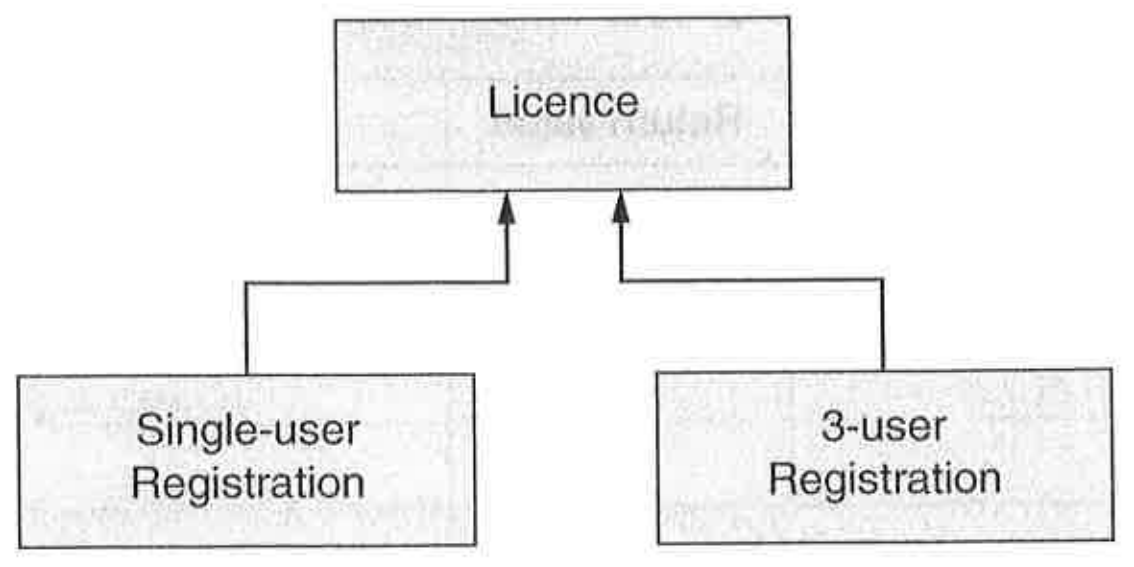
\includegraphics[width=0.5\paperwidth]{C:/Users/Admin/Desktop/Github/question_bank/LyX/static/img/9597-ALVL-2015-P1-Q3}
\par\end{center}

\subsubsection*{Task 3.5}

Write program code \textbf{only} for the three classes shown. 

Do not attempt to develop the application further.

\subsubsection*{Evidence 12}
\begin{itemize}
\item Program code for the three classes.\hfill{}{[}9{]}
\end{itemize}